\documentclass[11pt]{article}

%% MinionPro fonts 
%\usepackage[lf]{MinionPro}
%\usepackage{MnSymbol}
\usepackage{microtype}

%% Margins
\usepackage{geometry}
\geometry{verbose,letterpaper,tmargin=1in,bmargin=1in,lmargin=1in,rmargin=1in}

%% Other packages
\usepackage{amsmath}
\usepackage{amsthm}
\usepackage[shortlabels]{enumitem}
\usepackage{titlesec}
\usepackage{soul}
\usepackage{tikz}
\usepackage{mathtools}
\usepackage{pgfplots}
\usepackage{tikz-3dplot}
\usepackage{algorithmic}
\usepackage{optprog}
\usepackage[export]{adjustbox}
\usepackage{tcolorbox}

%% Paragraph style settings
\setlength{\parskip}{\medskipamount}
\setlength{\parindent}{0pt}

%% Change itemize bullets
\renewcommand{\labelitemi}{$\bullet$}
\renewcommand{\labelitemii}{$\circ$}
\renewcommand{\labelitemiii}{$\diamond$}
\renewcommand{\labelitemiv}{$\cdot$}

%% Colors
\definecolor{rred}{RGB}{204,0,0}
\definecolor{ggreen}{RGB}{0,145,0}
\definecolor{yyellow}{RGB}{255,185,0}
\definecolor{bblue}{rgb}{0.2,0.2,0.7}
\definecolor{ggray}{RGB}{190,190,190}
\definecolor{ppurple}{RGB}{160,32,240}
\definecolor{oorange}{RGB}{255,165,0}

%% Shrink section fonts
\titleformat*{\section}{\normalsize\bf}
\titleformat*{\subsection}{\normalsize\bf}
\titleformat*{\subsubsection}{\normalsize\it}

% %% Compress the spacing around section titles
\titlespacing*{\section}{0pt}{1.5ex}{0.75ex}
\titlespacing*{\subsection}{0pt}{1ex}{0.5ex}
\titlespacing*{\subsubsection}{0pt}{1ex}{0.5ex}

%% amsthm settings
\theoremstyle{definition}
\newtheorem{problem}{Problem}
\newtheorem{example}{Example}
\newtheorem*{theorem}{Theorem}
\newtheorem*{bigthm}{Big Theorem}
\newtheorem*{biggerthm}{Bigger Theorem}
\newtheorem*{bigcor1}{Big Corollary 1}
\newtheorem*{bigcor2}{Big Corollary 2}

%% tikz settings
\usetikzlibrary{calc}
\usetikzlibrary{patterns}
\usetikzlibrary{decorations}
\usepgfplotslibrary{polar}

%% algorithmic setup
\algsetup{linenodelimiter=}
\renewcommand{\algorithmiccomment}[1]{\quad// #1}
\renewcommand{\algorithmicrequire}{\emph{Input:}}
\renewcommand{\algorithmicensure}{\emph{Output:}}

%% Answer box macros
%% \answerbox{alignment}{width}{height}
\newcommand{\answerbox}[3]{%
  \fbox{%
    \begin{minipage}[#1]{#2}
      \hfill\vspace{#3}
    \end{minipage}
  }
}

%% \answerboxfull{alignment}{height}
\newcommand{\answerboxfull}[2]{%
  \answerbox{#1}{6.38in}{#2} 
}

%% \answerboxone{alignment}{height} -- for first-level bullet
\newcommand{\answerboxone}[2]{%
  \answerbox{#1}{6.0in}{#2} 
}

%% \answerboxtwo{alignment}{height} -- for second-level bullet
\newcommand{\answerboxtwo}[2]{%
  \answerbox{#1}{5.8in}{#2}
}

%% special boxes
\newcommand{\wordbox}{\answerbox{c}{1.2in}{.7cm}}
\newcommand{\catbox}{\answerbox{c}{.5in}{.7cm}}
\newcommand{\letterbox}{\answerbox{c}{.7cm}{.7cm}}

%% Miscellaneous macros
\newcommand{\tstack}[1]{\begin{multlined}[t] #1 \end{multlined}}
\newcommand{\cstack}[1]{\begin{multlined}[c] #1 \end{multlined}}
\newcommand{\ccite}[1]{\only<presentation>{{\scriptsize\color{gray} #1}}\only<article>{{\small [#1]}}}
\newcommand{\grad}{\nabla}
\newcommand{\ra}{\ensuremath{\rightarrow}~}
\newcommand{\maximize}{\text{maximize}}
\newcommand{\minimize}{\text{minimize}}
\newcommand{\subjectto}{\text{subject to}}
\newcommand{\trans}{\mathsf{T}}
\newcommand{\bb}{\mathbf{b}}
\newcommand{\bx}{\mathbf{x}}
\newcommand{\bc}{\mathbf{c}}
\newcommand{\bd}{\mathbf{d}}

%% LP format
%    \begin{align*}
%      \maximize \quad & \mathbf{c}^{\trans} \mathbf{x}\\
%      \subjectto \quad & A \mathbf{x} = \mathbf{b}\\
%                       & \mathbf{x} \ge \mathbf{0}
%    \end{align*}


%% Redefine maketitle
\makeatletter
\renewcommand{\maketitle}{
  \noindent SA405 

  \begin{center}\Large{\textbf{\@title}}\end{center}
}
\makeatother

%% ----- Begin document ----- %%
\begin{document}
\title{HW2: Intro to Network Models}

\maketitle

\textbf{1.} Graham Krackers has 3 plants where it produces (you guessed it) graham crackers that it then ships to 5 warehouses. The table below gives the plant and warehouse locations as well as the cost to ship between each plant and warehouse.

\begin{figure}[h!!!]
    \centering
    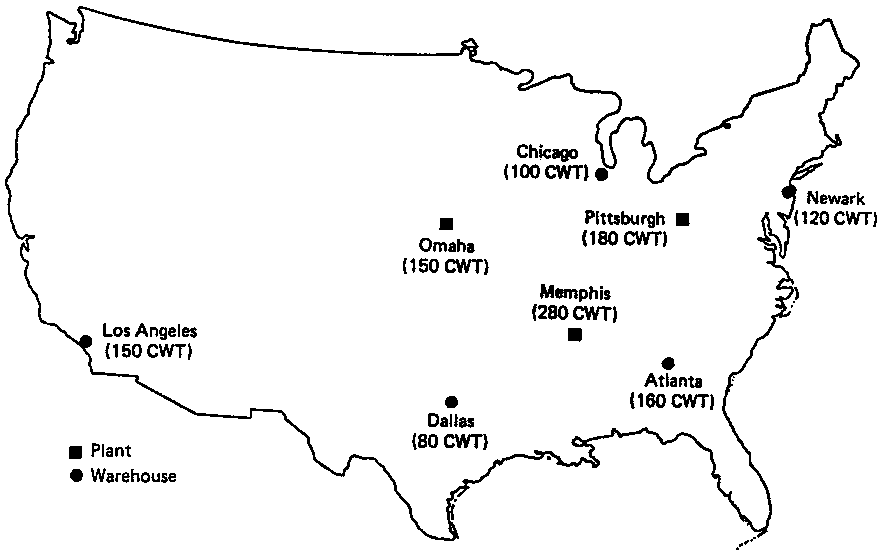
\includegraphics[width=4.3in]{map}\\
    \caption{Locations of Graham Krackers’ plants and warehouses}
\end{figure}

\begin{center}\begin{tabular}{|ccccccc|}\hline
  \$/ton   & Warehouse 1 & Warehouse 2 & Warehouse 3 & Warehouse 4 & Warehouse 5 &            \\
           &   (Newark) &  (Chicago) &  (Atlanta) &   (Dallas) & (Los Angeles) &   Supply   \\\cline{2-7}
   Plant 1 & \multicolumn{1}{|c|}{4} & \multicolumn{1}{|c|}{6} & \multicolumn{1}{|c|}{5} & \multicolumn{1}{|c|}{12} & \multicolumn{1}{|c|}{19} &    180 tons \\
(Pittsburgh) & \multicolumn{1}{|c|}{} & \multicolumn{1}{|c|}{} & \multicolumn{1}{|c|}{} & \multicolumn{1}{|c|}{} & \multicolumn{1}{|c|}{} &            \\ \cline{2-6}
   Plant 2 & \multicolumn{1}{|c|}{10} & \multicolumn{1}{|c|}{4} & \multicolumn{1}{|c|}{8} & \multicolumn{1}{|c|}{5} & \multicolumn{1}{|c|}{14} &    280 tons \\
 (Memphis) & \multicolumn{1}{|c|}{} & \multicolumn{1}{|c|}{} & \multicolumn{1}{|c|}{} & \multicolumn{1}{|c|}{} & \multicolumn{1}{|c|}{} &            \\ \cline{2-6}
   Plant 3 & \multicolumn{1}{|c|}{13} & \multicolumn{1}{|c|}{9} & \multicolumn{1}{|c|}{3} & \multicolumn{1}{|c|}{6} & \multicolumn{1}{|c|}{10} &    150 tons \\
   (Omaha) & \multicolumn{1}{|c|}{} & \multicolumn{1}{|c|}{} & \multicolumn{1}{|c|}{} & \multicolumn{1}{|c|}{} & \multicolumn{1}{|c|}{} &            \\ \cline{1-6}
   Demand &    120 tons &    100 tons &    160 tons &     80 tons &    150 tons &            \\ \hline
\end{tabular}\end{center}

\begin{enumerate}
\item[a)] Draw the network diagram for this problem.
\item[b)] Formulate a concrete model that would allow Graham Krackers to satisfy demand of the warehouses at minimum cost.
\item[c)] Formulate a parameterized model that would allow Graham Krackers to satisfy demand of the warehouses at minimum cost.
\end{enumerate}

\newpage

\textbf{2.} (slightly modified problem 2.36 from the book) Velvet Ale is produced by a local brewer. Currently, it has three production plants in town, one that can produce 1000 bottles a day, another that produces 750 bottles per day, while the third produces only 500 bottles per day. The brewer uses two distributors to deliver its beer to the three stores that sell it. The (per day) demand for the three stores is 700, 600, and 800, respectively. In addition, cost (in cents per bottle) to ship the beer between locations is given in the table below.

\begin{center}
\begin{tabular}{c|ccccc} \hline
& Distributor 1 & Distributor 2 & Store 1 & Store 2 & Store 3 \\ \hline
Plant 1 & 8 & 14 & - & - & - \\
Plant 2 & 12 & 10 & - & - & - \\
Plant 3 & 16 & 12 & - & - & - \\
Distributor 1 & - & - & 10 & 8 &  12 \\
Distributor 2 & - & - & 6 & 15 & - \\ \hline
\end{tabular}

\end{center}

\begin{enumerate}
\item[a)] Draw the network diagram for this problem.
\item[b)] Formulate a concrete model that would allow the brewer to satisfy demand at minimum cost.
\item[c)] Formulate a parameterized model that would allow the brewer to satisfy demand at minimum cost.
\end{enumerate}





\end{document}
